% 开题报告模板:不超过一页
\documentclass[conference]{IEEEtran}

\pagestyle{plain}


\usepackage{todonotes}
\usepackage{fontspec,xltxtra,xunicode}
%\usepackage{threeparttable}
\usepackage{listings}
%\usepackage{titlesec}
%\usepackage{fontspec} % 定制字体
\usepackage{xcolor} % 定制颜色
\definecolor{mygreen}{rgb}{0,0.6,0}
\definecolor{mygray}{rgb}{0.5,0.5,0.5}
\definecolor{mymauve}{rgb}{0.58,0,0.82}
\lstset{ %
backgroundcolor=\color{white},      % choose the background color
%basicstyle=\footnotesize\ttfamily,  % size of fonts used for the code
basicstyle=\small\ttfamily,  % size of fonts used for the code
columns=fullflexible,
tabsize=2,
breaklines=true,               % automatic line breaking only at whitespace
captionpos=b,                  % sets the caption-position to bottom
commentstyle=\color{mygreen},  % comment style
escapeinside={\%*}{*)},        % if you want to add LaTeX within your code
keywordstyle=\color{blue},     % keyword style
stringstyle=\color{mymauve}\ttfamily,  % string literal style
%frame=single,
rulesepcolor=\color{red!20!green!20!blue!20},
% identifierstyle=\color{red},
%language=Java,
mathescape
}


\defaultfontfeatures{Mapping=tex-text}
%\setromanfont{Heiti} %设置中文字体
\setromanfont{SimSun} %设置中文字体

\XeTeXlinebreaklocale “zh”
\XeTeXlinebreakskip = 0pt plus 1pt minus 0.1pt %文章内中文自动换行,可以自行调节

\newfontfamily{\Song}{SimSun} %设定新的字体快捷命令
%\newfontfamily{\E}{Weibei} %设定新的字体快捷命令
\newfontfamily{\kai}{KaiTi} %设定新的字体快捷命令
\newfontfamily{\hei}{SimHei} %设定新的字体快捷命令

%\titleformat*{\section}{\hei}
%\titleformat*{\subsection}{\hei}

%%%%%% 设置字号 %%%%%%
\newcommand{\chuchuhao}{\fontsize{48pt}{\baselineskip}\selectfont}
\newcommand{\chuhao}{\fontsize{42pt}{\baselineskip}\selectfont}
\newcommand{\xiaochuhao}{\fontsize{36pt}{\baselineskip}\selectfont}
\newcommand{\yihao}{\fontsize{28pt}{\baselineskip}\selectfont}
\newcommand{\erhao}{\fontsize{21pt}{\baselineskip}\selectfont}
\newcommand{\xiaoerhao}{\fontsize{18pt}{\baselineskip}\selectfont}
\newcommand{\sanhao}{\fontsize{15.75pt}{\baselineskip}\selectfont}
\newcommand{\sihao}{\fontsize{14pt}{\baselineskip}\selectfont}
\newcommand{\xiaosihao}{\fontsize{12pt}{\baselineskip}\selectfont}
\newcommand{\dawuhao}{\fontsize{11.5pt}{\baselineskip}\selectfont}
\newcommand{\wuhao}{\fontsize{10.5pt}{\baselineskip}\selectfont}
\newcommand{\xiaowuhao}{\fontsize{9pt}{\baselineskip}\selectfont}
\newcommand{\liuhao}{\fontsize{7.875pt}{\baselineskip}\selectfont}
\newcommand{\qihao}{\fontsize{5.25pt}{\baselineskip}\selectfont}

\renewcommand\refname{参考文献}
\renewcommand{\abstractname}{{\hei 摘要}}

%%%% 下面的命令设置行间距与段落间距 %%%%
\linespread{1.2}
% \setlength{\parskip}{1ex}
\setlength{\parskip}{0.5\baselineskip}


%%% 插图, Figure --> 图
\renewcommand{\figurename}{图}
\renewcommand{\tablename}{表}


%indent
\makeatletter
\let\@afterindentfalse\@afterindenttrue
\@afterindenttrue
\makeatother
\setlength{\parindent}{2em}  %中文缩进两个汉字位


\begin{document}
%
% paper title
% can use linebreaks \\ within to get better formatting as desired
\title{反$2D$欺骗攻击面部活性检测}


% author names and affiliations
% use a multiple column layout for up to three different
% affiliations
\author{\IEEEauthorblockN{}
\IEEEauthorblockA{孙添琦\\
tqsun@mail.ustc.edu.cn}
\and
\IEEEauthorblockN{第9组}
\IEEEauthorblockA{孙铁\\
kyles@mail.ustc.edu.cn}
\and
\IEEEauthorblockN{}
\IEEEauthorblockA{汤鑫\\
tangx@mail.ustc.edu.cn}
}

% make the title area
\maketitle

\iffalse
% 中文摘要
\begin{abstract}
论文摘要。。。
\end{abstract}

\vskip.2cm

% 中文关键词
\renewcommand{\abstractname}{{\hei 关键词}}
\begin{abstract}
关键词1;关键词2;关键词3;关键词4
\end{abstract}

\vskip.2cm

% 中图法分类号
\renewcommand{\abstractname}{{\hei 中图法分类号}}
\begin{abstract}
TP319
\end{abstract}

\vskip.2cm

% 英文摘要
\renewcommand{\abstractname}{Abstract}
\begin{abstract}
Abstract in English...
\end{abstract}

\vskip.2cm

% 英文关键词
\renewcommand{\abstractname}{Keywords}
\begin{abstract}
Keywords 1,Keywords 2,Keywords 3,Keywords 4
\end{abstract}
\fi

\section{引言}

\subsection{研究背景}
生物识别技术技术已广泛应用于个人识别领域。与密码等传统的安全方法相比,生物识别技术利用人的内在特征进行个体识别带来了方便。
人脸识别是最常见的生物特征之一,因为无需任何物理接触就可以很容易地从人脸中提取信息。它已经在许多个人识别应用中得到了成功的演示。

当今社会人脸识别已经得到了广泛应用,然而传统的人脸识别系统往往没有考虑恶意攻击者的存在。
攻击者可以伪装成系统授权的人,从而获得对系统的非法访问。
比较典型的例子是2D欺骗攻击,它通过使用有效用户的二维面部副本来迷惑系统,是一种最常见的攻击方法。

\subsection{问题分析}
二维欺骗攻击主要有三种类型:照片攻击、视频攻击和模拟面具攻击。
照片攻击通过在一张纸上或电子屏幕上使用合法用户的照片来逃避检测;
而视频攻击通过在电子设备上通过播放授权人员的视频来迷惑系统;
在模拟面具攻击中,对手戴着一个二维面具伪装成授权人员。

人脸活跃度检测,又称人脸欺骗检测,是为了抵御二维欺骗攻击而设计的活体检测手段。
通常意义上的活体检测是当生物特征信息从合法用户那里取得时,判断该生物信息是否从具有生物活体的合法用户身上取的。
活体检测的方法主要是通过识别活体上的生理信息来进行,它把生理信息作为生命特征来区分用照片、硅胶、塑料等非生命物质伪造的生物特征。
人脸活跃度检测可以在人脸识别过程开始前确定图像是来自真实的还是虚假的主体。可疑图像会被过滤,而不会被传送到识别系统。

\section{相关工作}
人脸活度检测可分为基于软件和基于硬件两种方式。
以往人脸活度检测的工作主要集中在基于软件的方法上,通过分析被试的纹理、结构信息、活度标志以及所捕获图像的质量等数据来进行判别检测。
这些方法通常对环境因素敏感,比如在光照条件差、图像噪声大等情况下,检测精度会明显下降。
此外,某些活动性线索的计算复杂度较高,如基于连续帧的人脸动态计算。
虽然要求用户说话或摇头可以提高检测的准确性,但由于检测时间较长且用户不一定配合,也会降低检测效率。

基于硬件的方法则是通过在识别系统中嵌入设备来获取被测试者的额外信息,比如红外检测仪器,温度检测仪器等。
虽然嵌入这些设备会让分析更为准确,但是设备安装往往较为麻烦且费用昂贵,大大增加了检测成本。

\section{系统架构设计与实现}
本研究阐述了一个利用闪光灯进行人脸活性检测的模型,以抵御照片、视频以及模拟面具攻击。
本课题采用基于软硬件结合的方法,对比合法用户和恶意用户的图像差异,通过硬件设备闪光灯放大差异;
针对性地设计人脸信息的特征描述符,提取特征值;
获取特征之后使用支持向量机 $SVM$ 进行训练,得到训练模型。

\subsection{输入}
本次研究需要使用代表合法用户和三种$2D$攻击的四种检测对象:
合法用户,合法用户的照片,合法用户的视频,戴着合法用户的面具的攻击者。
在检测过程中从对象上获取闪光灯开启前后的一对图像。
\vskip.4cm
\centerline
{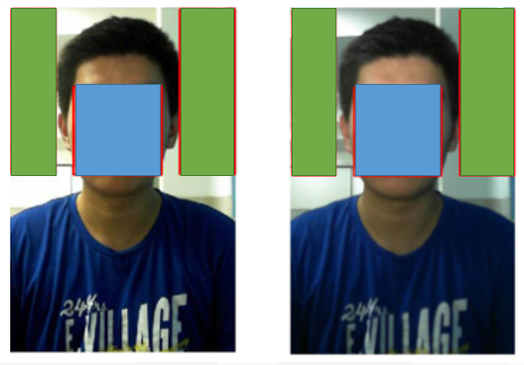
\includegraphics[width=0.33\textwidth]{p1.png}}
\centerline{\small 图1 \ \ 摄像头获取的原始待处理图像}

针对获取的原始待处理图像,主要处理三个区域:蓝色区域代表脸部区域$I_F$;
绿色区域代表背景区,为分布在左上角和右上角的两个矩形区域$I_{BR}$和$I_{BL}$,统称为$I_B$。

\subsection{特征描述符}
\subsubsection{特征描述符$LBP \_ FI$}
\ 

局部二值模式$LBP$对光照具有良好的鲁棒性,十分契合我们的需求,所以选择使用$LBP$算法来获取面部纹理特征。

将人脸区域$I_F$分成$9$个不重叠的块,每块为一个算子。为了获取图像不同区域的纹理信息,需要计算每个算子中像素的$LBP$码。

原始的$LBP$算子定义为一个 $3*3$ 像素的窗口。
以窗口中心像素的灰度值为阈值,将相邻的8个像素的灰度值与其进行比较,若周围像素值大于中心像素值,则该像素点的位置被标记为$1$,否则为$0$。
这样,$3*3$邻域内的8个点经比较可产生一个$8$位二进制数,转换为十进制数即得到该窗口中心像素点的$LBP$值,这个值可以用来反映该区域的纹理信息。

\vskip.4cm
\centerline
{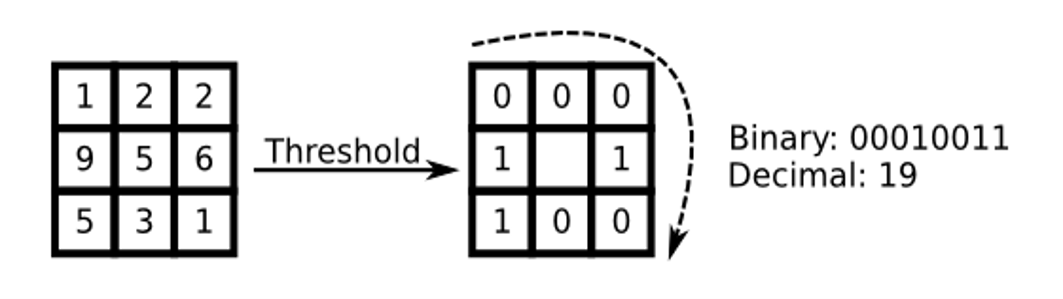
\includegraphics[width=0.33\textwidth]{p2.png}}
\centerline{\small 图2 \ \ 局部二值模式$LBP$}
\ 
计算公式:

\ \ {$LBP(x_c,y_c) = \displaystyle\sum_{i = 0}^{7}s(p_i-p_c)\times 2^{i}.$}

由于采用传统$LBP$模式的统计直方图来表达图像的信息时,较多的模式种类将使得需要处理分析的数据量过大(一个拥有 $P$ 个采样点的$LBP$算子将会产生 $2^{p}$ 种模式),同时也会使直方图过于稀疏。
因此,就需要对原始的LBP模式进行降维,使得数据量减少的情况下依然能代表图像的信息。
为了解决二进制模式过多的问题,提高统计性,$T.Ojala$ 提出了采用一种“等价模式”来对$LBP$算子的模式种类进行降维。
将优化之后降维的$LBP$算法称为等价$LBP$算法($Uniform \ LBP$)。

当某个$LBP$算子所对应的循环二进制数最多有两次从$0$到$1$或从$1$到$0$的跳变时,该$LBP$算子所对应的二进制被视为等价模式类;
除等价模式类以外的模式都被归为一个模式,称为混合模式类。这使得二进制模式的种类大大减少,但并不会丢失任何信息。
模式数量由原来的 $2^{p}$ 种减少为 $P\times (P-1)+3$ 种。特征向量的维数更少,减少了高频噪声带来的影响。

根据各个算子区域计算得到的 $LBP(x_c, y_c)$ 生成统计直方图$H_i$。
等价模式$LBP$算法中每个$3*3$算子生成的直方图有$59$项,其中$58$种等价模式类分别表示为$1\sim58$,混合模式类表示为$0$,$9$个统计直方图共有 $59*9=531$ 项。
统计直方图连接成为一个向量,也就是整幅图像的LBP纹理特征向量。

\ \ {$LBP \_ FI = (H1,H2,H3,\dots,H9).$}

特征描述符 $LBP \_ FI$ 是用来从图片的纹理等信息上进行面部活性检测,类似于传统的基于软件的检测方法。

接下来则是需要使用机器学习的方法,针对合法用户和恶意攻击进行二分类,通过$OpenCV$将提取的特征进行$SVM$训练。

\ 

\subsubsection{特征描述符$SD \_ FIC$}
\ 

我们将人脸区域$I_F$在闪光灯亮起前后的灰度值变化的标准差$\sigma_{D^{F}}$作为第二个特征描述符 $SD \_ FIC$。

计算公式:

{$SD \_ FIC = \sigma_{D^{F}} = \displaystyle\sqrt{\frac{\sum_{i=1}^{N}{(D^{F}(x_i,y_i)-\mu_{D^{F}})}^{2}}{N-1}}.$}

\ 

\ \ {$D^{F}(x_i,y_i) = I_f^{F} - I_n^{F}.$}

\ 

\ \ {$\mu_{D^{F}} = {\displaystyle\frac{\sum_{i=1}^{N}(D^{F}(x_i,y_i))}{N}}.$}

\ 

$I_n^{F}$ 与 $I_f^{F}$ 分别为 $I_F$ 在闪光灯亮起前后的灰度值;

$N$ 指待理图像的像素数量;

$D^{F}(x_i,y_i)$ 为 $I_F$ 在闪光灯亮起前后的灰度值差;

$\mu_{D^{F}}$ 为 $I_F$ 在闪光灯亮起前后灰度值变化平均值。

特征描述符 $SD \_ FIC$ 反映的是由闪光灯引起的人脸区域 $I_F$ 灰度强度变化。
由于闪光灯的照射距离、光照强度等结构信息不同,其照射到真实人脸上不同的部位所产生的光反射效果也必然会不同。

二维欺骗攻击往往是一个平面图像,相比真实人脸的反射光会更加均匀,也就是说闪光灯照射前后真实人脸的灰度强度变化偏差会大于二维欺骗攻击的灰度强度偏差。
所以我们考虑利用标准差来捕捉模型中灰度强度的变化。

三维物体上的灰度强度变化明显区别于二维,所以真实人脸的 $SD \_ FIC$ 值在所有情况中会是最大的;
而纸照片攻击、二维面具攻击和曲面面具攻击产生的图像会在闪光灯亮起时在人脸区域出现明亮的光带,也因此比其他类型的二维欺骗攻击有更大的 $SD \_ FIC$。


\subsubsection{特征描述符$M \_ BIC$}
\ 

我们将背景区域$I_{BR}$和$I_{BL}$在闪光灯亮起前后的灰度值变化的平均值$\mu_{D^{BG}}$作为第三个特征描述符 $M \_ BIC$。

\ 
计算公式:

{$M \_ BIC$ = $\mu_{D^{BG}} = {\displaystyle\frac{\sum_{i=1}^{N}(D^{F}(x_i,y_i))}{N}}.$}

\ 

\ \ {$D^{BG}(x_i,y_i) = I_f^{BG} - I_n^{BG}.$}

\ 

$I_n^{BG}$ 与 $I_f^{BG}$ 分别为 $I_B$ 在闪光灯亮起前后的灰度值;

$N$ 指待理图像的像素数量;

$D^{BG}(x_i,y_i)$ 为 $I_B$ 在闪光灯亮起前后的灰度值差;

实际背景在图片攻击和视频攻击中会被遮盖,这也就使得从视频设备上捕获的背景比实际的背景离摄像头更近。
因此当闪光灯照射到视频攻击时会反射出更高强度的光,我们可以利用$M \_ BIC$来捕捉这些信息。

由于真实人脸和面具攻击都不会遮盖真实背景,而真实背景在使用了闪光灯的图像中会被闪光灯遮挡,
这就导致它们相比照片攻击和视频攻击的$M \_ BIC$要小得多;

\subsubsection{特征描述符$SD \_ BIC$}
\ 

我们将背景区域$I_{BR}$和$I_{BL}$在闪光灯亮起前后的灰度值变化的标准差$\sigma_{D^{BG}}$作为第三个特征描述符 $SD \_ BIC$。

\ 
计算公式:

{$SD \_ BIC = \sigma_{D^{BG}} = \displaystyle\sqrt{\frac{\sum_{i=1}^{N}{(D^{BG}(x_i,y_i)-\mu_{D^{F}})}^{2}}{N-1}}.$}

\ 

\ \ {$D^{BG}(x_i,y_i) = I_f^{BG} - I_n^{BG}.$}

\ 

$I_n^{BG}$ 与 $I_f^{BG}$ 分别为 $I_B$ 在闪光灯亮起前后的灰度值;

$N$ 指待理图像的像素数量;

$D^{BG}(x_i,y_i)$ 为 $I_B$ 在闪光灯亮起前后的灰度值差;

虽然面具攻击和真实人脸都不会遮盖实际背景,但由于纹理和形状不同,面具的光扩散效果会不同于真实的脸。

面具的光扩散要比人脸的光扩散大,真实人脸的$SD \_ BIC$值会小于面具攻击的$SD \_ BIC$值。

由于视频和照片的二维平面结构,闪光灯会让视频攻击和纸质照片攻击中背景区域的强度增加。这些攻击的$SD \_ BIC$会比不覆盖真实背景的攻击要小。

\subsubsection{期望}
\ 

依据各个特征描述符的性质进行分析,我们期望实验测试所得到的数据效果应该表现出

\ 1. 所有攻击都要比真实人脸的$SD \_ FIC$小很多;

\ 2. 照片和视频要比真实人脸的$M \_ BIC$大很多;

\ 3. 面具和真实人脸的$M \_ BIC$相差不大;

\ 4. 照片和视频要比真实人脸的$SD \_ BIC$小;

\ 5. 面具要比真实人脸的$SD \_ BIC$大。

期望函数:

\ \ ${C = \displaystyle(\frac{SD \_ FIC}{M \_ BIC})^{(1+\left | SD \_ BIC-SD \_ BIC_n \right|)}.}$

$SD \_ BIC_n$为真实人脸作为输入时的$SD \_ BIC$的数学期望。

\section{实验结果与分析}
\subsection{实验环境}
选取合法用户、合法用户的纸质照片、合法用户的电子照片($1024*768$ 像素)、合法用户的视频($1024*768$ 像素)、
合法用户的$2D$面具、合法用户的卷曲面具六种输入。

自然光照度大约等于$40lx$。设置的闪光灯照度为$200lx$。

拍摄对象和摄像头之间的距离是$0.60$米。闪光灯设置在摄像头的正上方。


\subsection{实验数据}

分别得到三种结构信息特征描述符如下:

{
\begin{table}[h]
    \centering
    \begin{tabular}{l r r r}
        \hline
                    & $\ SD \_ FIC$ & $\ M \_ BIC$ & $\ SD \_ BIC$ \\ \hline
        真实人脸     & 39.45       & 36.88      & 24.02   \\ 
        纸质照片     & 19.42       & 62.12      & 25.81   \\ 
        电子照片     & 18.52       & 58.87      & 17.13   \\ 
        视频         & 17.03       & 63.24      & 13.11   \\ 
        $2D$ 面具    & 30.44       & 35.57      & 37.76   \\ 
        卷曲面具     & 33.80       & 43.88      & 33.88   \\ \hline
    \end{tabular}
\end{table}   
}

可以看出,实验数据完全符合期望。

通过运行时间和常用的半总错误率$HTER$准则来进行各种活度检测方法的性能比较,$HTER$越小说明性能表现越好。
下图给出了本方法和其他现有检测方法的$HTER$,加粗的数字为当前列的最小值:
\vskip.4cm
\centerline
{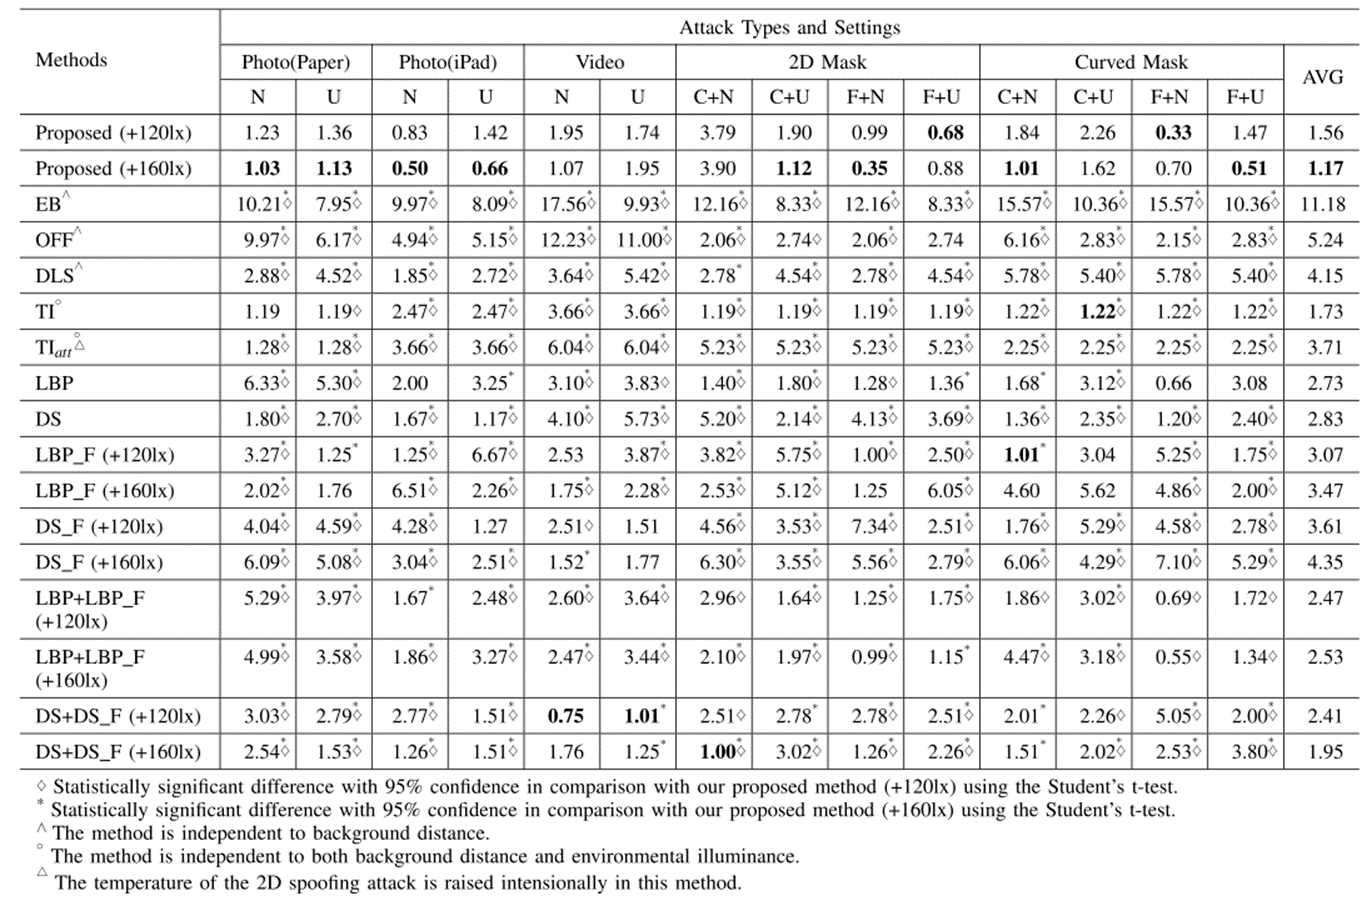
\includegraphics[width=0.50\textwidth]{p3.png}}
\centerline{\small 图3 \ \ 各种活性检测方法的$HTER$表}

从上图可以看出,本研究所阐述的软硬件结合的活性检测算法在照片攻击和模拟面具攻击上表现为最优,在视频攻击上也极为接近最优水平。
而其他方法大多受到各种条件的制约。

\subsection{分析总结}
$LBP \_ FI$ 描述符捕获纹理信息进行人脸的面容识别;
$SD \_ FIC$、$M \_ BIC$ 和 $SD \_ BIC$ 三种描述符测量结构信息,进行活性检测。
四个特征描述符都有各自侧重的攻击领域,综合起来可以区别各种二维攻击。

闪光灯与自然光相比具有更强的照明度,放大了真假人脸的差别且有效减少了环境因素的影响。


\section{总结与展望}

本研究阐述了一种基于软硬件相结合的人脸活性检测二维欺骗攻击的方法。
根据四种特征描述符测量的闪光灯图像的差异,将被试分为合法类和恶意类。
与基于硬件的方法不同,此方法只需要闪光灯,既经济实惠且又易于安装在现有的人脸识别系统中。
由于闪光灯增强了真假人脸的差别,减少了环境光照的影响,因此该方法比单纯的基于软件的方法更准确、鲁棒性更强。
此外,提取四个描述符的时间复杂度较低,不需要用户协作。
此方法既利用了基于软件的方法,又利用了基于硬件的方法。
具有精度高、鲁棒性强、计算复杂度低、安装成本低等优点。

文中方法也有一定的局限性,比如对闪光灯的距离有严格要求,而且闪光灯的位置要对用户友好。
虽然部分型号的闪光灯的照度对人眼没有伤害,也远低于相机使用闪光灯的照度,但是用户的舒适度是一个问题。
一种可能的解决办法是调整闪光角度。如果不将闪光灯安装在眼睛的高度,闪光灯的照射就不会直接刺激人眼,反而会让人感觉更舒适。
闪光灯设备角度的确定不仅要依据检测精度,还要依据安装难度等因素。

这一研究未来的工作可能是专注于探索模型的性能,使之可以对更先进的攻击进行检测防御,比如3D欺骗攻击,即精良的3D人脸面具和3D模型的各种表情。
由于表面反射率的不同,真实人脸和3D面具的反射光是不同的,此外3D的纹理细节也可以通过闪光灯来增强。
因此,如果能够找出合适的描述符,额外的闪光灯照明也应该依然有助于将合法用户与恶意攻击区分开来。


\begin{thebibliography}{99}

    \bibitem{D}
    D  Wen,  Han H ,  Jain A K . 
    Face Spoof Detection With Image Distortion Analysis[J]. 
    IEEE Transactions on Information Forensics \& Security, 2015, 10(4):746-761.
    
    \bibitem{chan}
    Chan P ,  Liu W ,  Chen D , et al. 
    Face Liveness Detection Using a Flash Against 2D Spoofing Attack[J]. 
    IEEE Transactions on Information Forensics \& Security, 2018, 13(2):521-534.

    \bibitem{Ojala}
    Ojala T , Pietikainen M , Maenpaa T .
    Multiresolution Gray-Scale and Rotation Invariant Texture Classification with Local Binary Patterns[J].
    IEEE Transactions on Pattern Analysis and Machine Intelligence, 2002, 24(7):971-987.

    \bibitem{taotao}
    taotao1233.
    LBP特征学习及其实现.
    https://blog.csdn.net/jinshengtao/article/details/18219697.
    2014.

    \bibitem{qianqing}
    qianqing13579.
    LBP特征的实现及LBP + SVM分类.
    https://blog.csdn.net/qianqing13579/article/details/49406563.
    2015.

\end{thebibliography}

\end{document}






